%%==================================================================%%
%% Author : Sa�udo Olmedo, Ignacio                                  %%
%%          S�nchez Barreiro, Pablo                                 %%
%% Version: 1.3, 18/06/2014                                         %%
%%                                                                  %%
%% Memoria del Proyecto Fin de Carrera                              %%
%% Antecedentes, archivo ra�z                                       %%
%%==================================================================%%

\chapterheader{Antecedentes y Planificaci�n}{Antecedentes y Planificaci�n}
\label{chap:background}

Este cap�tulo describe las tecnolog�as y t�cnicas utilizadas en el desarrollo del presente Proyecto de Fin de Carrera. La primera secci�n est� dedicada a introducir el caso de estudio del PFC presentado, el cual consiste en la realizaci�n de un generador de c�digo Cassandra que transforma modelos UML a modelos escritos en Cassandra. La siguiente secci�n est� dedicada a describir en qu� consiste EMF el lenguaje utilizado para desarrollar lenguajes de modelado.  A continuaci�n se describe la herramienta Epsilon que se ha utilizado para desarrollar el generador de c�digo. La siguiente secci�n est� dedicada a explicar de manera breve algunos conceptos de Cassandra. Finalmente se expone la planificaci�n que ha seguido el proyecto para su realizaci�n, desde formaci�n hasta desarrollo.

\chaptertoc

\section{Introducci�n}
\label{sec:back:introduccion}

%%==================================================================%%
%% Author : Abascal Fern�ndez, Patricia                             %%
%% Author : S�nchez Barreiro, Pablo                                 %%
%% Version: 1.2, 24/06/2013                                         %%
%%                                                                  %%
%% Memoria del Proyecto Fin de Carrera                              %%
%% Application Engineering/Introduccion                             %%
%%==================================================================%%

Este cap�tulo describe el proceso de desarrollo de los generadores de c�digo para la segunda fase del desarrollo de una l�nea de productos software (ver Figura~\ref{back:fig:domainAplicEng}), el proceso de \emph{Ingenier�a de Aplicaciones}. El objetivo de esta fase, tal como comentamos, es obtener productos concretos y funcionales a partir de la composici�n, configuraci�n y personalizaci�n de los elementos creados en la fase de \emph{Ingenier�a del Dominio}. 
 
Para ello, de acuerdo con la metodolog�a Te.Net (ver Secci�n~\ref{sec:intr:tenet}), el primer paso es crear una selecci�n de aquellas caracter�sticas que se desea incluir en el producto, de acuerdo a las necesidades particulares de cada clientes. C�mo se crea dicha selecci�n de caracter�sticas est� fuera del �mbito de este proyecto. Referimos al lector interesado al Proyecto Fin de Carrera de D. Daniel Tejedo, antiguo alumno de esta Facultad~\citep{}.

Una vez obtenida una selecci�n de caracter�sticas v�lida, utilizando dicha selecci�n, se configura la arquitectura de referencia creada en la fase de \emph{Ingenier�a del Dominio} para crear un modelo arquitect�nico concreto, adaptado a las necesidades del cliente, del producto que queremos construir.  Dicho modelo arquitect�nico se obtiene de forma autom�tica mediante la utilizaci�n del lenguaje \emph{VML}~\citep{}, de acuerdo con la metodolog�a Te.Net (ver Secci�n~\ref{sec:intr:tenet}). Una descripci�n detallada del lenguaje VML tambi�n est� fuera del �mbito de este proyecto, y referimos al lector interesado a los trabajos de~\cite{} y~\cite{}.

Este modelo arquitect�nico de un product concreto es el que sirve de entrada al generador de c�digo que queremos desarrollar. Utilizando dicho modelo como entrada, el generador de c�digo debe producir todo el c�digo necesario para componer las clases parciales creadas a nivel de \emph{Ingenier�a del Dominio} que correspondan. Para ello debe generar las clases parciales encargadas de llevar a cabo tal composici�n, las versiones limpias de los m�todos requeridos, y las delegaciones a las versiones sucias adecuadas. 

Para ello, el primer paso era dise�ar un algoritmo que permitiese calcular estos tres elementos: (1) clases parciales requeridas; (2) versiones limpias necesarias; y, (3) delegaciones adecuadas. A continuaci�n, deb�amos implementar este algoritmo utilizando plantillas de generaci�n de c�digo, por lo que deb�amos, igual que en cap�tulo anterior, prestar especial atenci�n a su secuenciaci�n. 

Por �ltimo, deb�amos dise�ar y realizar las pruebas que permitiesen comprobar el correcto funcionamiento del generador de c�digo. Tras estas pruebas, se daba por concluido el proceso de desarrollo de los generadores de c�digo, y procedimos a su despliegue. 

Para explicar este proceso de desarrollo, este Cap�tulo se estructura como sigue: La Secci�n~\ref{application:sec:alg} describe la estructura de los modelos de entrada que nuestro generador de c�digo debe procesar. La Secci�n~\ref{application:sec:alg} describe el dise�o del algoritmo encargado de calcular los elementos a componer, de acuerdo al modelo de entrada proporcionado. La Secci�n~\ref{application:sec:transf} explica c�mo se han secuenciado las plantillas de generaci�n de c�digo para poder implementar dicho algoritmo. La Secci�n~\ref{application:sec:pruebas} describe el proceso de dise�o y ejecuci�n de las pruebas para el generador de c�digo implementado. Por �ltimo, la Secci�n~\ref{application:sec:despliegue} detalla las acciones realizadas durante la fase de despliegue de la aplicaci�n.








\section{Caso de estudio: Generador de c�digo CQL-Cassandra}
\label{sec:back:casoEstudio}

%%==========================================================================%%
%% Author : Sa�udo Olmedo, Ignacio                                          %%
%% Author : S�nchez Barreiro, Pablo                                         %%
%% Version: 1.2, 21/04/2014                                                 %%
%%                                                                          %%
%% Memoria del Proyecto Fin de Carrera                                      %%
%% M2M/Caso de estudio                                                      %%
%%==========================================================================%%

Como se explicaba en el capitulo 2 en la secci�n "Caso de estudio" el objetivo de este caso de estudio es la creaci�n de un generador de c�digo de una versi�n simplificada de Twitter.
En esta secci�n se reproducir�n los procesos M2M y M2T en el siguiente capitulo, todo esto bajo el proceso de desarrollo dirigido por modelos. Esta secci�n esta dedicada a describir la transformaci�n del modelo UML de Twissandra a un modelo Cassandra. Partiendo del modelo UML de la figura~\ref{back:fig:twissandra} y una vez establecidas las reglas de transformaci�n entre modelos, esta secci�n explica el proceso de transformaci�n del modelo UML al modelo Cassandra.

En primer lugar, marcamos el atributo username de la clase User como clave. En el caso de la clase FollowingRelationship y la clase Tweet al no tener un atributo marcado como clave generamos una clave sustituta autom�ticamente para cada clase, llamadas FollowingRelationship\_id y tweet\_id respectivamente.

Por cada paquete estereotipado como <<dataModel>>, se crea un nuevo keyspace. El nombre del keyspace ser� el nombre utilizado por el data model. Los atributos restantes de las meta-clases del keyspace se establecen en sus valores definidos por defecto. A continuaci�n, todos los elementos correspondientes de ese paquete se procesan y se colocan dentro de su keyspace correspondiente.

Como se mencionaba en las reglas de transformaci�n, la clase User se transforma en una Column Family llamada User. A continuaci�n, los atributos y las asociaciones se procesan. Por �ltimo, el atributo Username, que se marc� como clave en el modelo de datos UML, es marcado como Primary Key. De manera similar para aquellos atributos del modelo UML cuya multiplicidad sea igual a uno se realiza una transformaci�n simple, por ejemplo el atributo username y password se transforman en dos columnas, ambos del tipo text. Estas columnas est�n contenidas en la column family User. De la misma manera se transforman los atributos body y time de la clase Tweet y el atributo timestamp de la clase FollowingRelationship.
En el caso de el atributo del modelo UML email cuya multiplicidad es mayor de uno y tiene las propiedades isUnique establecida en false y la propiedad isOrdered establecida en false (en el modelo no se puede apreciar pero esta configurado as�), se transforma este atributo en un set llamado email de tipo text dentro de la column family User.

En cuanto a las asociaciaciones de multiplicidad igual a uno la transformaci�n que se realiza por ejemplo, para la asociaci�n de la clase user una nueva columna llamada user\_username (recordemos que username es la clave de la column family user) es creada y a�adida a la column family Tweet. Para las asociaciones cuya multiplicidad es mayor de uno, por ejemplo la asociaci�n llamada userline se crea una dynamic column family llamada User\_userline. A continuaci�n una columna llamada user\_username de tipo text es a�adida a esta column family. Despu�s una columna llamada tweet\_id de tipo uuid es a�adida (el atributo tweet\_id fue creado en la column family tweet al no tener clave). Las columnas user\_username y tweet\_id son designadas como primary key, la columna user\_username ser� la partition key. 

\section{EMF}
\label{sec:back:EMF}

%%==================================================================%%
%% Author : Sa�udo Olmedo, Ignacio                                  %%
%%          S�nchez Barreiro, Pablo                                 %%
%% Version: 1.3, 18/06/2014                                         %%
%%                                                                  %%
%% Memoria del Proyecto Fin de Carrera                              %%
%% Background/EMF                                                   %%
%===================================================================%%
Para comenzar el desarrollo del proyecto bajo el paradigma del desarrollo software dirigido por modelos necesitamos definir que lenguajes de modelado vamos a utilizar. En el cap�tulo anterior coment�bamos que es necesario definir el lenguaje de modelado que utilizara Cassandra para ello usaremos EMF. Eclipse Modeling Framework (EMF) (\cite{dave:2008}) es un framework de modelado que nos proporciona la base para la elaboraci�n de lenguajes de modelado. Para la creaci�n de meta-modelos EMF (\cite{kolovos:2014}) utiliza dos modelos de meta-datos: \emph{Ecore} y \emph{Genmodel}. Ecore contiene la informaci�n sobre las clases que se han definido. Genmodel contiene informaci�n adicional para la generaci�n del c�digo, por ejemplo la ruta y la informaci�n del archivo. Genmodel tambi�n contiene atributos que sirven de control a la hora de generar el c�digo, encontramos los siguientes par�metros de control:
\begin{enumerate}
\item EClass: representa una clase, con cero o m�s atributos y cero o m�s referencias.
\item EAttribute: representa un atributo que tiene un nombre y un tipo.
\item EReference: representa un extremo de una asociaci�n entre dos clases.
\item EDataType: representa el tipo de un atributo, por ejemplo, int, float.
\end{enumerate}
Estos atributos nos servir�n a la hora de crear las reglas de transformaci�n entre modelos UML y modelos Cassandra.

Utilizando EMF se pueden crear meta-modelos de forma gr�fica muy similar a los diagramas de clases en UML.
EMF permite crear un meta-modelo a trav�s de diferentes medios, por ejemplo, XMI, anotaciones Java, XML o UML. Adem�s EMF proporciona un framework para almacenar la informaci�n del modelo.
Un ejemplo sencillo de la utilidad de EMF es el siguiente: Imaginemos que deseamos construir una aplicaci�n para manipular mensajes escritos en XML. El primer paso que dar�amos ser�a empezar definiendo el schema del mensaje sin embargo con EMF se puede trabajar ignorando este nivel. Con EMF podemos crear plugins que generen por ejemplo un diagrama de clases UML a partir de este mensaje XML o directamente generar el c�digo Java que implemente las clases del mensaje XML.




\section{Epsilon}
\label{sec:back:epsilon}

%%==================================================================%%
%% Author : Sa�udo Olmedo, Ignacio                                  %%
%%          S�nchez Barreiro, Pablo                                 %%
%% Version: 1.1, 18/06/2014                                         %%
%%                                                                  %%
%% Memoria del Proyecto Fin de Carrera                              %%
%% Background/Epsilon                                               %%
%===================================================================%%


Epsilon es una familia de lenguajes y herramientas para el desarrollo de software dirigido por modelos, entre estas herramientas podemos encontrar: herramientas de transformaci�n de modelos, validaci�n de modelos o generaci�n de c�digo entre otras funcionalidades. Epsilon es distribuido a trav�s de la plataforma de modelado de lenguajes de Eclipse.
Epsilon proporciona multitud de lenguajes y herramientas para trabajar con modelos. Los lenguajes utilizados en este proyecto son \emph{EOL} (Epsilon Object Language), \emph{ETL} (Epsilon Transformation Language) y \emph{EGL} (Epsilon Generation Language) tambi�n ha sido utilizado \emph{EUnit} como herramienta para validar el c�digo escrito por el generador de c�digo Cassandra-CQL. Estos lenguajes y herramientas son descritos a continuaci�n. Toda la informaci�n sobre estos lenguajes as� como su utilizaci�n ha sido obtenida de (\cite{kolovos:2014})

\subsection{Epsilon Object Language}
\emph{Epsilon Object Language} (EOL) es un lenguaje de programaci�n imperativo utilizado para crear, consultar y modificar los modelos EMF. EOL se puede considerar un lenguaje mezcla de Javascript y OCL, que combina lo mejor de ambos lenguajes. Como tal, proporciona todas las caracter�sticas habituales imperativas que se encuentran en Javascript (por ejemplo, la secuencia de la declaraci�n, las variables, bucles for y while, etc) y todas las caracter�sticas interesantes de OCL como las operaciones sobre colecciones, por ejemplo Sequence\{1..5\}.select(x \textbar\ x \textgreater\ 3).


\begin{figure}[!tb]
  \centering
  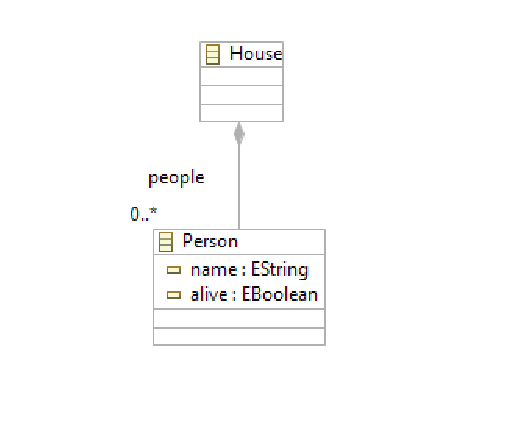
\includegraphics[width=.8\linewidth]{background/images/ejCasa.eps} \\
  \caption{Ejemplo metamodelo casa}
  \label{back:fig:ejMetamodeloCasa}
\end{figure}


Para entender mejor el funcionamiento de EOL se expone el siguiente ejemplo. Se ha definido el meta-modelo mostrado en la figura~\ref{back:fig:ejMetamodeloCasa}, este meta-modelo consiste en la representaci�n de una casa y las personas que viven en ella. Las personas tienen un nombre y un atributo booleano que representa si una persona est� viva o no. Existe una relaci�n de agregaci�n para reflejar que la casa contiene personas.
Una vez creado el meta-modelo podemos crear un modelo como instancia de ese meta-modelo. Un ejemplo de c�mo funciona EOL puede ser el siguiente: deseamos saber que personas habitan en la casa y est�n vivas. La sintaxis correspondiente ser�a la siguiente (figura~\ref{back:code:codigoEOL}).

\begin{figure}[!tb]
\begin{center}
\begin{footnotesize}
\begin{verbatim}
--------------------------------------------------------
for (person in Person.all){
  if (person.alive == true) {
    person.name.println();
  }
}

//Podemos realizar lo mismo de la siguiente manera:

Person.all.select(r|r.alive==true).name.println();

--------------------------------------------------------
\end{verbatim}
\end{footnotesize}
\end{center}
\caption{Ejemplo c�digo EOL}
\label{back:code:codigoEOL}
\end{figure}


Como vemos la sintaxis es muy similar a cualquier lenguaje orientado a objetos, podemos manipular y consultar los objetos del modelo, sin embargo EOL no nos permite la definici�n de clases.


\subsection{Epsilon Transformation Language}
\emph{Epsilon Transformation Language} (ETL) es un lenguaje de transformaci�n modelo a modelo basado en reglas (\imp{Model to Model-M2M}). ETL proporciona las caracter�sticas est�ndar de un lenguaje de transformaci�n, tambi�n nos permite manipular los modelos de entrada y salida as� como su c�digo fuente. ETL tiene su propia sintaxis sin embargo utiliza el lenguaje EOL como base.


Recordando el ejemplo de la Red de computadores y el Grafo detallado en el capitulo anterior (secci�n 1.2). Deseamos realizar la transformaci�n de un modelo de tipo grafo a un modelo de tipo red para ello definiremos una serie de reglas de transformaci�n utilizando para ello ETL. En primer lugar necesitamos definir el modelo del grafo para poder realizar la transformaci�n a un modelo de tipo Red.
La figura~\ref{back:code:codigoETL} muestra el c�digo que realiza el proceso de transformaci�n de un Grafo a una Red.

\begin{figure}[!tb]
\begin{center}
\begin{footnotesize}
\begin{verbatim}

rule Arista2Cable
transform a : Grafo!Arista
to r : Red!Cable {	
    r.nameCable = a.nombreArista;
    if (a.parent.isDefined()) {
        r.parent=Red;
        for (nodoArista in a.children) {
            if(nodoArista.color=TColor#R){
                var PC : new Red!PC;
                PC.nameNodo="PC"+iPC;
                r.children.add(PC);
                iPC=iPC+1;	
            }
            else{
                var Router : new Red!Router;
                Router.nameNodo="Router"+iRouter;
                r.children.add(Router);
                iRouter=iRouter+1;
            }
        }
    }	
}

\end{verbatim}
\end{footnotesize}
\end{center}
\caption{Ejemplo c�digo ETL}
\label{back:code:codigoETL}
\end{figure}

En este c�digo encontramos solo una regla. Esta regla transforma aristas del grafo a cables de la red. La primera instrucci�n copia el nombre de la arista al cable. A continuaci�n la primera condicional cuestiona si esa arista tiene un padre definido en caso afirmativo asigna el cable a la red. A continuaci�n por cada nodo se crea o bien un PC o un router dependiendo del color del nodo que se est� analizando (rojo-PC, azul-Router). En siguiente lugar se asigna el nodo creado al cable correspondiente y finalmente se a�ade a la red. Este proceso se repite por cada arista del grafo. Una vez ejecutado este c�digo dado un modelo de entrada de tipo Grafo obtenemos un modelo equivalente de tipo Red que cumple las reglas definidas en el meta-modelo.


\subsection{Epsilon Generation Language}

\emph{Epsilon Generation Language} (EGL) (\cite{louis:2008}) es un lenguaje utilizado para la generaci�n de c�digo basado en la transformaci�n de modelos (\imp{Model to Text-M2T}).
EGL puede ser utilizado para transformar modelos en cualquier tipo de lenguaje, por ejemplo c�digo ejecutable Java, c�digo HTML o incluso aplicaciones completas que comprenden el c�digo en varios lenguajes (por ejemplo, HTML, Javascript y CSS). En este proyecto se utilizara EGL para la generaci�n de c�digo Cassandra Query Language (CQL) a partir de modelos UML 2.0.

Cada plantilla de EGL contiene varias secciones. Cada secci�n puede ser est�tica o bien din�mica.
Una secci�n est�tica contiene texto que aparecer� en la salida generada por la plantilla. Una secci�n din�mica comienza con la secuencia '[\%' y termina con la secuencia '\%]'. La secci�n din�mica contiene lenguaje EOL.
La figura~\ref{back:code:codigoEGL} muestra como se realiza la generaci�n de c�digo HTML utilizando para ello el modelo generado de una red a partir de un grafo (ver secci�n anterior).

\begin{figure}[!tb]
\begin{center}
\begin{footnotesize}
\begin{verbatim}
--------------------------------------------------------
[%
    var red: Red := Red.allInstances().at(0);
%]

<html>
    <head>
        <title> Red </title>
    </head>
    <body>
        <h1>Conexiones</h1>				
        <table  border="1">
            <col style="width: 200px" />
            <col style="width: 100px" span="3" />
            [% for (conexiones in red.conexiones){%]
            <tr>
                <th scope="row">[%=conexiones.nameCable%]</th>
                [% for (nodos in conexiones.children){%]
                    <td>[%=nodos.nameNodo%]</td>
                [%	}%]
            </tr>
            [%	}%]
        </table>
    </body>
</html>
--------------------------------------------------------
\end{verbatim}
\end{footnotesize}
\end{center}
\caption{Ejemplo c�digo EGL}
\label{back:code:codigoEGL}
\end{figure}

Como vemos en el c�digo la integraci�n del c�digo EGL junto con HTML es total, en este sencillo c�digo se genera una p�gina HTML con una tabla que muestra varias filas, una fila por cada conexi�n entre dos componentes de la red. 

\section{Cassandra}
\label{sec:back:cassandra}

%%==================================================================%%
%% Author : Sa�udo Olmedo, Ignacio                                  %%
%%          S�nchez Barreiro, Pablo                                 %%
%% Version: 1.1, 18/06/2014                                         %%
%%                                                                  %%
%% Memoria del Proyecto Fin de Carrera                              %%
%% Background/Cassandra                                             %%
%===================================================================%%
http://www.nosql-database.org/
[chalmers]
%http://www.acens.com/wp-content/images/2014/02/bbdd-nosql-wp-acens.pdf
%http://www.strozzi.it/cgi-bin/CSA/tw7/I/en_US/NoSQL/Philosophy%20of%20NoSQL
Desde que naci� SQL en el a�o 1974, SQL ha sido el modelo de base de datos relacionales utilizado por excelencia. En los �ltimos a�os ha surgido otra vertiente denominada NoSQL la cual surge por la necesidad de manejo de grandes vol�menes de informaci�n no estructurada, distribuida con la mayor rapidez posible. NoSQL es usado en plataformas como Facebook o Twitter. Podemos encontrar varios tipos de bases de datos no relacionales; Bases de datos documentales, bases de datos clave-valor, orientadas a grafos y mas tipos.

Las principales caracter�sticas de NoSQL que difieren de SQL son:
\begin{enumerate}
\item NoSQL no garantiza las propiedades ACID (atomicidad, coherencia, aislamiento y durabilidad).
\item No utiliza SQL como lenguaje de consultas. Algunas bases de datos no relacionales utilizan SQL como lenguaje de apoyo sin embargo la mayor�a utilizan su propio lenguaje de consultas como por ejemplo Cassandra que utiliza CQL.
\item No est� permitido el uso de joins ya que al manejar grandes vol�menes de informaci�n una consulta con un join puede llegar a sobrecargar el sistema.
\item Escalan horizontalmente y trabajan de manera distribuida por lo que la informaci�n puede estar en distintas maquinas y el a�adir nodos mejora el rendimiento.
\item Resuelven problemas de altos vol�menes de informaci�n
\end{enumerate}

En este proyecto de fin de carrera se utiliza Cassandra, Cassandra es una distribuci�n de bases de datos no relaciones (NoSQL). Dentro del mundo de las bases de datos no relaciones Cassandra pertenece a la familia de bases de datos denominada "clave-valor". Las bases de datos clave-valor son aquellas que  asocian los valores a una determinada clave esto permite la recuperaci�n y escritura de informaci�n de forma muy r�pida y eficiente. Cassandra re�ne las  tecnolog�as de sistemas distribuidos de Amazon Dynamo y el modelo de datos BigTable de Google. Al igual que Dynamo, Cassandra es consistente. Como BigTable, Cassandra proporciona un modelo de datos basado en ColumnFamily siendo considerado el sistema basado en clave-valor m�s popular.

Las bases de datos basadas en Cassandra son soluciones utilizadas cuando es necesaria escalabilidad y alta disponibilidad sin comprometer el rendimiento. Escalabilidad lineal y tolerancia a fallos o infraestructura en la nube lo convierten en la plataforma perfecta para datos de misi�n critica. Cassandra proporciona gran estabilidad en cuanto a la replicaci�n de datos a trav�s de m�ltiples datacenters, consiguiendo una menor latencia para sus usuarios y la tranquilidad de que no existan perdidas de datos ante ca�das. Cassandra utiliza un lenguaje llamado CQL (Cassandra Query Language) con una sintaxis muy similar a SQL aunque con menos funcionalidades.

Fue dise�ado por Avinash Lakshman (uno de los creadores de Amazon's Dynamo) y Prashant Malik (Ingeniero de Facebook). Cassandra est� en producci�n para Facebook sin embargo aun est� en fase de desarrollo.

%https://cassandra.apache.org/ http://www.datastax.com/documentation/cql/3.0/cql/ddl/ddl_intro_c.html

A continuaci�n se explican algunos t�rminos que hay que tener en cuenta cuando se trabaja con Cassandra.
En Cassandra un KeySpace es el equivalente a una base de datos en los sistemas de bases de datos relacionales. El conocido t�rmino de tabla en las bases de datos relacionales tiene su equivalente en Cassandra llamado Column Family. Por lo tanto un KeySpace puede contener varias Column Families y una Column Family a su vez contiene varias columnas.
Una columna es la unidad de almacenamiento b�sica, est� formada de tres campos: Nombre, un valor y un timestamp. El nombre y el valor se almacena como una matriz de bytes sin procesar y pueden ser de cualquier tama�o. Un ejemplo:
Nombre de la columna 	\"Username\"
Nombre de usuario	\"Ignacio\"
Timestamp 		\"123456789\"
La sintaxis del lenguaje CQL es muy similar a SQL, CQL contiene sintaxis ya conocida de SQL como INSERT, DELETE, UPDATE, INSERT,  ...
Un ejemplo de c�digo CQL ejecutable es el siguiente (Figura~\ref{back:code:codigoCQL})


\begin{figure}[!tb]
\begin{center}
\begin{footnotesize}
\begin{verbatim}

DROP KEYSPACE twitter;

CREATE KEYSPACE twitter
WITH replication = {'class':'SimpleStrategy', 'replication_factor':2};

USE twitter;

CREATE TABLE Tweet(
       UUID text,
       usernameTw text,
       body text,
       PRIMARY KEY(UUID)
);

CREATE TABLE User(
       username text,
       password text,
       followers set<text>,
       followings set<text>,
       tweets_written list<text>,
       PRIMARY KEY(username)
);

\end{verbatim}
\end{footnotesize}
\end{center}
\caption{Ejemplo c�digo CQL}
\label{back:code:codigoCQL}
\end{figure}




\section{Planificaci�n}
\label{sec:back:planificacion}

%%==================================================================%%
%% Author : Sa�udo Olmedo, Ignacio                                  %%
%%          S�nchez Barreiro, Pablo                                 %%
%% Version: 1.2, 18/06/2013                                         %%
%%                                                                  %%
%% Memoria del Proyecto Fin de Carrera                              %%
%% Background/Planificacion                                         %%
%===================================================================%%

El objetivo de este proyecto de fin de carrera es la implementaci�n de un generador de c�digo Cassandra a partir de modelos UML. El proceso de desarrollo as� como el de aprendizaje que se ha seguido para la realizaci�n del proyecto es descrito a continuaci�n.

La primera tarea como es evidente consisti� en adquirir los conocimientos necesarios para el desarrollo del proyecto, en primer lugar todo lo relacionado con el proceso de modelado de un lenguaje y transformaci�n de lenguajes [kleppe]. Tambi�n fueron necesarios conocimientos sobre la Ingenier�a y el Desarrollo Dirigido por Modelos, as� como de la sintaxis, arquitectura y funcionamiento de Cassandra.

A continuaci�n se comenz� a trabajar con la herramienta Epsilon, sus lenguajes EOL, EGL, ETL y EUnit como herramienta para las pruebas de los modelos y c�digo generados. As� como con el lenguaje para la definici�n de lenguajes de modelado Eclipse Modeling Framework (EMF).
Para conocer c�mo funcionaban estos lenguajes se desarrollaron una serie de casos pr�cticos para familiarizarse con los m�todos de transformaci�n as� como con la herramienta, para ello se realizo el proceso completo para crear un generador de c�digo desde la transformaci�n entre modelos hasta la transformaci�n modelo-c�digo. Estos casos de prueba son los que se exponen en la secci�n de Epsilon.

Una vez conocido estos conceptos se estudiaron las reglas de transformaci�n a aplicar para transformar un modelo UML a un modelo Cassandra, estas reglas fueron propuestas por [pabloCassandra].

Tras estas tareas de adquisici�n de conocimientos se empez� a trabajar en el generador de c�digo Cassandra empezando por la transformaci�n de modelos UML a modelos Cassandra. Estas transformaciones son expuestas en el siguiente cap�tulo. Una vez finalizada la transformaci�n se comenz� a trabajar en el generador de c�digo Cassandra, esta tarea es descrita en el cap�tulo 5. Tras realizar dicha tarea se realizaron una serie de casos de prueba para verificar si los resultados que otorgaba el generador de c�digo eran los esperados, para esta tarea utilizamos la herramienta EUnit.

Finalmente y tras generar varios casos de ejemplo se instalo la plataforma de Cassandra BLABLA 

\section{Sumario}
\label{sec:back:sumario}

%%==================================================================%%
%% Author : Abascal Fern�ndez, Patricia                             %%
%%          S�nchez Barreiro, Pablo                                 %%
%% Version: 1.1, 21/06/2013                                         %%
%%                                                                  %%
%% Memoria del Proyecto Fin de Carrera                              %%
%% Antecedentes, Sumario                                            %%
%%==================================================================%%

Durante este cap�tulo se han descrito los conceptos necesarios para comprender el �mbito y el alcance de este proyecto. Se ha descrito el caso de estudio que se utilizar� a lo largo del documento. A continuaci�n, se ha especificado qu� es una l�nea de productos software, el dise�o orientado a caracter�sticas, la metodolog�a TENTE, las limitaciones de las clases parciales en C\#, c�mo pueden resolverse estas limitaciones mediante el uso del \emph{SlicerPattern} y el proceso de generaci�n de c�digo con Epsilon.

